\documentclass[class=report, crop=false, a4paper, 12pt]{standalone}

%Packages import
\usepackage{../pkgs}


\begin{document}
\par From the previously described systems in Section~\ref{sec:related_work}, it is possible to infer that a DL approach can be grouped in two implementation choices: the methods of 1) face detection and 2) face representation (that include the feature extracting backbone neural network and the loss function necessary for training\footnote{As this dissertation specifically concentrates on the face recognition domain, the loss function pertains exclusively to the training of that stage.}). The next sections describe the choices of those and reasons behind them, as well as the implementation and steps necessary for that effect.

\section{Face detection}
\par Following the proposed pipeline for a Face Recognition system, the initial design choice pertains to the Face Detection module, responsible for detecting, selecting and standardizing the faces. A comprehensive study of solutions was presented in Section 2.3.1, wherein RetinaFace emerged as the best overall solution for a student monitoring context. This approach accepts an image as input and produces multiple outputs, including a bounding box, five key facial landmarks (representing the center of the eyes, nose, and corners of the mouth), and a confidence score that reflects the likelihood of the detection accurately identifying a face. The selection of this option was predominantly influenced by three critical factors: 1) Adaptability to changes in light, pose, facial expressions, etc., facilitated by the DCNN backbone, 2) incorporation of a single-stage approach and leveraging multi-task learning, enabling efficient real-time detection of facial landmarks using just a single CPU core (for VGA resolution), and 3) availability of readily implemented solutions with ample support.

\par The implementation of choice is a Pytorch implementation\footnote{\url{https://github.com/biubug6/Pytorch_Retinaface}} of the original code that offers both a MobileNet-0.25 or ResNet-50 as backbones pre-trained on ImageNet. To better suit our application, further development over the original code was needed. RetinaFace is distributed as a general face detection algorithm that's deployed on data with multiple faces to be handled, therefore, there's no built-in methods for face selection or transformations, like alignment and resizing. However, on a student's monitoring scenario, only one face is relevant, and as consequence of that, the face recognition systems are to be trained and validated on single face pictures normalized to a canonical view.

\begin{figure}[!h]
    \centering
    \includegraphics[width=0.9\textwidth]{RF_1_crop.jpg}
    \caption{Results produced by the RetinaFace method over a test photo. Represented are the bounding boxes, respective confidence scores and the five facial landmarks.}
    \label{fig:rf_1}
\end{figure}

\newpage
Instantiating the model with default threshold parameters and Resnet-50 as the backbone, it produces the results seen in \reffig{fig:rf_1}. From all the bounding boxes available, one must be picked, and one way of doing so is by assuming that the more relevant face is closer to the camera, hence the area of its bounding box will be greater.

\begin{figure}[h]
    \centering
    \begin{minipage}[c]{0.48\textwidth}
      \centering
      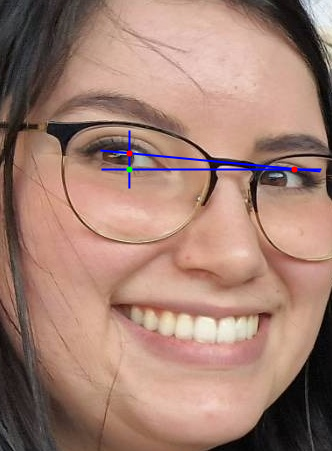
\includegraphics[width=0.9\textwidth]{RF_2.png}
      \label{fig:rf_2}
    \end{minipage}
    \hfill
    \begin{minipage}[c]{0.48\textwidth}
      \centering
      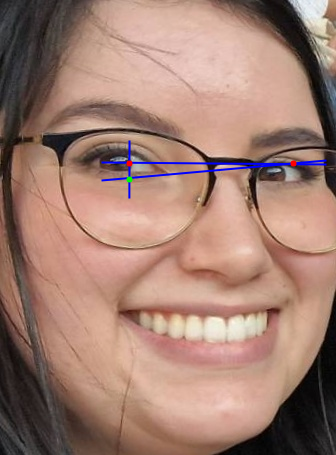
\includegraphics[width=0.9\textwidth]{RF_3.png}
      \label{fig:rf_3}
    \end{minipage} 
    %\vspace{-0.4cm}
    \caption{Landmark based alignment. The green dot serves as an auxiliary point, resulting from the intersection of a horizontal line originating at the pivot eye and a vertical line projected from the other eye. Subsequently, the rotation angle is determined by computing the arctangent of two distances: the distance between the higher eye and the auxiliary point, and the distance from the auxiliary point to the pivot eye.}
    \label{fig:rf_2_3}
\end{figure}

\par The alignment is done with the help of the eyes landmarks as seen in \reffig{fig:rf_2_3}. The eye lower relative to the other is declared as the pivot and starting point of a horizontal line that acts as the reference to calculate the angle of rotation. Following the selection, cropping, and alignment of the face, it is resized to fit the required dimensions for the subsequent phase.

\section{Face Representation}
The Face Representation stage has the task of handling the features of each face and includes a feature extractor and a loss function. Following the review on related works in Section~\ref{sec:related_work} Ganidisastra and Bandung~\autocite{ganidisastraIncrementalTrainingDeep2021} and SMOWL~\autocite{labayenOnlineStudentAuthentication2021} both utilize Facenet trained with triplet loss for face recognition. This naturally prompts an investigation into the potential effects on performance when utilizing a more modern network (ResNet variations), as well as a lightweight network with fewer parameters (MobileFaceNet). Furthermore, considering the drawbacks associated with triplet loss training, examining the impact of a well-established loss function, like ArcFace, which encourages intra-class compactness and inter-class distance, would also be noteworthy. Due to time constraints, the methods of choice are all pretrained and subsequently finetuned on datasets appropriate to the model's scenario deployment.

\subsection{FaceNet}
For this method, we utilize a highly regarded PyTorch implementation\footnote{https://github.com/timesler/facenet-pytorch} that offers pretrained models in either the CASIA-WebFace or VGGFace2 dataset. The images' faces are cropped and aligned (but not rotated) using MTCNN, and resized to $160\times160\times3$. However, this implementation has differences compared to the Facenet described in the original paper~\autocite{schroffFaceNetUnifiedEmbedding2015}. Firstly, differing from the original adopted GoogLeNet-style Inception model, the backbone network employed here is the Inception Resnet V1, which integrates residual blocks into the Inception architecture. As highlighted in Section~\ref{sec:resnet}, this modification streamlines the training process by addressing issues such as accuracy degradation and gradient vanishing. Secondly, adhering to the recommendations by Parkhi \textit{et al.}~\autocite{parkhiDeepFaceRecognition2015}, the network was trained as a classifier using softmax loss, departing from the original's triplet loss metric learning approach. Finally, the method's output is a 512-dimensional embedding, differing from the 128-dimensional output reported in the original paper.

\subsection{ResNet}
The choices for this architecture we're designed to cover a range of neural network depth, complexity and trainable parameters. Henceforth, there are 3 objects of study, ranging from less to deeper ones: iResnet-18 \footnote{\url{https://github.com/deepinsight/insightface}}, Resnet-34 \footnote{\red{link needed}} (from the TrustID project) and iResnet-50 (with Squeeze and Excitation blocks)\footnote{\label{fnote6}\url{https://github.com/TreB1eN/InsightFace_Pytorch}}. Both the iResnet-18 and iResnet-50 were trained on $112\times112\times3$ faces from the MS1MV2 dataset, using ArcFace as the loss function, and output 512-dimensional feature embeddings. Regarding the Resnet-34, it was trained with triplet loss on a custom dataset comprised of 3 million $150\times150\times3$ images from the Visual Geometry Group
Face~\autocite{parkhiDeepFaceRecognition2015} and FaceScrub~\autocite{ngDatadrivenApproachCleaning2014}, and outputs a 128-dimensional feature embedding.

\subsection{MobileFaceNet}
MobileFaceNet \cref{fnote6} is the lightscale approach to face recognition that will further aid the study of the computational cost and model's performance trade-off. Being that is made available by the same author as the iResnet-50, it has technical similarities. Once again, it is trained with ArcFace loss on $112\times112\times3$ images from the MS1MV2 dataset and outputs the usual 512-dimensional embedding.


\section{Finetuning data}
Considering that the intended application of the face recognition systems is to monitor students, it is not unreasonable to assume that, due to the nature of the capture device (webcam or smartphone) or its positioning, that will be reflect on the quality of the data. For instance, one potential scenario involves a student with one monitor and a laptop placed to the side of it, accompanied by a lamp on the opposite side. This will configuration will result in face captures with very different resolutions, poses and lightning compared to another student using a laptop, against a well lit window, facing the subject. Therefore, it is crucial to have a robust system that is capable of being insensitive to these variations, hence the possible need to finetune pretrained models for that. In this regard, we will examine two distinct datasets: DigiFace-1M and QMUL-SurvFace.
\par Amidst the controversies surrounding the methods of data acquisition for some publicly distributed datasets, including MS-Celeb-1M, MegaFace, FaceScrub, IJB-C or VGGFace, Bae \textit{et al.} developed DigiFace-1M~\autocite{baeDigiFace1MMillionDigital2023} with those concerns in mind. This fully synthetic dataset emulates different scenarios with variant poses, light, expression and accessories (hats, masks, makeup, etc.), and it serves as an interesting object of study of the potential of this type of datasets to diminish the reliance over real face data to finetune a model for more adverse scenarios.
\par The second dataset used to finetune our models of choice is QMUL-SurvFace~\autocite{chengSurveillanceFaceRecognition2018} by Cheng \textit{et al.}. Initially described as a benchmarking dataset, its unconstrained way of capturing resulted on faces with very high variance in resolution, capturing angles, poses, light or accessories, poses as a perfect source to further adapt the models to said scenarios. Another noteworthy benefit of this dataset is that the images we're collected with the consent of the individuals, meaning that ethical and privacy dilemmas are not at play.

\section{Benchmarks}
\section{Implementation details}
\par All the training, processing, and benchmarking code was developed in a Docker environment to ensure reproducibility. The code was written using Python 3.8.10 and relies on PyTorch 1.14.0 and Torchvision 0.15.0, along with their corresponding required libraries. The training process is conducted exclusively on a single GPU, specifically NVIDIA's GeForce RTX 3080 Ti, using Optuna\footnote{\url{https://optuna.org/}} as an automatic hyperparameter optimization tool.
\par All the codes were developed with modularity in mind. First, the data is processed with the custom RetinaFace algorithm and saved. Then, it is proceeded forward to the neural network that produces a feature embedding for each image. If the model is being trained (finetuned in our case), the embedding will be passed on to the ArcFace module, which will output the feature's logits \red{I might need to explain what logits are}. Following the original paper, the logits must be turned to probabilities by applying the softmax activation function and then contributing to the final step, i.e, the cross entropy loss. This is handled by Pytorch's function \red{CrossEntropyLoss}, since it performs both steps simultaneously. Because ArcFace is a separate structure that does not integrate the backbone networks as a custom layer, the neural networks can be quickly and easily changed.


\end{document}



